\documentclass[12pt]{article}
\usepackage{multicol}
\usepackage{cite}

\usepackage{graphicx}
\usepackage[doublespacing]{setspace}
\usepackage[hidelinks]{hyperref}
\usepackage{titlesec}
\newcommand{\sectionbreak}{\clearpage}

\usepackage[dvipsnames]{xcolor}
\usepackage{listingsutf8}

% From: https://gordonlesti.com/custom-code-highlighting-in-latex/

\lstdefinelanguage{Dockerfile}
{
  morekeywords={FROM, RUN, CMD, LABEL, MAINTAINER, EXPOSE, ENV, ADD, COPY,
    ENTRYPOINT, VOLUME, USER, WORKDIR, ARG, ONBUILD, STOPSIGNAL, HEALTHCHECK,
    SHELL},
  morecomment=[l]{\#},
  morestring=[b]"
}


\newcommand\YAMLcolonstyle{\color{red}\mdseries}
\newcommand\YAMLkeystyle{\color{black}\bfseries}
\newcommand\YAMLvaluestyle{\color{blue}\mdseries}

% From: https://tex.stackexchange.com/questions/152829/how-can-i-highlight-yaml-code-in-a-pretty-way-with-listings

\makeatletter

% here is a macro expanding to the name of the language
% (handy if you decide to change it further down the road)
\newcommand\language@yaml{yaml}

\expandafter\expandafter\expandafter\lstdefinelanguage
\expandafter{\language@yaml}
{
  keywords={true,false,null,y,n},
  keywordstyle=\color{darkgray}\bfseries,
  basicstyle=\YAMLkeystyle,                                 % assuming a key comes first
  sensitive=false,
  comment=[l]{\#},
  morecomment=[s]{/*}{*/},
  commentstyle=\color{purple}\ttfamily,
  stringstyle=\YAMLvaluestyle\ttfamily,
  moredelim=[l][\color{orange}]{\&},
  moredelim=[l][\color{magenta}]{*},
  moredelim=**[il][\YAMLcolonstyle{:}\YAMLvaluestyle]{:},   % switch to value style at :
  morestring=[b]',
  morestring=[b]",
  literate =    {---}{{\ProcessThreeDashes}}3
                {>}{{\textcolor{red}\textgreater}}1     
                {|}{{\textcolor{red}\textbar}}1 
                {\ -\ }{{\mdseries\ -\ }}3,
}

% switch to key style at EOL
\lst@AddToHook{EveryLine}{\ifx\lst@language\language@yaml\YAMLkeystyle\fi}
\makeatother

\newcommand\ProcessThreeDashes{\llap{\color{cyan}\mdseries-{-}-}}

\lstset{basicstyle=\linespread{0.5}\ttfamily,
  showstringspaces=false,
  commentstyle=\color{red},
  keywordstyle=\color{blue},
  inputencoding=utf8,
  extendedchars=true
}

\lstset{frame=tb,
  aboveskip=8mm,
  columns=flexible,
  numbers=none,
  tabsize=3
}

\graphicspath{{./images/}}

\author{Sammy Furr}
\title{The Development of a Collaborative Tool to Teach Debugging}
\date{\today}

\begin{document}

\begin{titlepage}
  \maketitle
\end{titlepage}

\begin{abstract}
  TODO: write an abstract
\end{abstract}

\tableofcontents
\pagebreak

\section{Introduction}

The goal of this project is to create a collaborative debugger to aid
in the teaching of debugging.  The collaborative debugger aims to help
teachers integrate this undertaught skill into their classes.  It
realizes the benefits of collaborative programming and teaching
debugging by providing a platform that is genuinely useful to students
and teachers.

\subsection{Motivation}

Debugging is invaluable in writing and understanding code, yet it is
rarely formally taught\cite{doi:10.1080/08993400802114581}.  We
typically teach students programming structures, concepts, and
languages, but leave them to learn the tools they use to write code by
themselves.  This approach often works well---a programmer's choice of
tools is often \textit{very} personal and students figure out how to
configure an individualized workflow.  Perhaps because debuggers are
tools, students are often expected to learn them with minimal
guidance.  Unlike editors or reference guides however, effectively
using a debugger requires a set of high-level, platform agnostic,
teachable skills.  Teaching these skills is effective, and translates
into better, faster, debugging and
programming\cite{10.1145/3286960.3286970}\cite{10.1145/3361721.3361724}.
Teaching these debugging skills collaboratively will likely offer the
same confidence and correctness benefits realized by teaching
programming collaboratively
\cite{10.1145/1026487.1008043}\cite{10.1145/1145287.1145293}.

\subsubsection{The Value of Teaching Debugging}

There is an unfortunate lack of research specifically into the
efficacy of teaching debugging for computer science students, despite
a recent rise in the inclusion of debugging in ``computational
thinking'' curriculums\cite{10.1145/3361721.3361724}.  These
curriculums attempt to teach skills in computer science classes that
translate into other subject areas: the UK's computer science
curriculum considers debugging an essential ``transferable
skill''\cite{10.1145/2602484}.\par

There seems to be confidence that the problem-solving techniques used
in debugging are widely applicable, but of greater interest to
computer science teachers is whether teaching debugging directly
benefits student programmers.  Michaeli and Romeike conducted a good,
albeit somewhat small, study on the efficacy of teaching a systematic
debugging process to K12 students.  They found that students who have
been taught a specific debugging framework performed better in
debugging tests and were more confident in their own debugging
skills\cite{10.1145/3361721.3361724}.  Their result is positive
evidence towards the efficacy of teaching debugging, though it doesn't
include college or university students.\par

As Michaeli and Romeike point out, there is a lack of research into
the value of teaching debugging in higher education.  None of the
research these authors found placed much focus on explicitly teaching
debugging.  Chmiel and Loui studied whether students who were provided
with debugging tools and frameworks performed better on tests or spent
less time on assignments than those who were
not\cite{10.1145/971300.971310}.  Though this research wasn't able to
find conclusive evidence towards better performance on tests or
assignments, it did find that students in the treatment group felt
more confident in their debugging abilities.  Unfortunately Chmiel and
Loui's study didn't involve extended explicit teaching of
debugging---use of the tools was voluntary, and variations in the
students' individual abilities made the data difficult to
evaluate.\par

Though there is a lack of higher-education research, the value of
teaching debugging is still demonstrable.  The research discussed all
finds that K-12 and college students alike commonly resort to sporadic
debugging techniques when beginning to learn.  Since this pattern of
behavior that explicitly teaching debugging corrects exists in college
as well as in K-12 students, it seems logical that the benefit of
explicitly teaching debugging to K-12 students should be realized
equally by their collegiate counterparts.\par

\subsubsection{Methods for Teaching Debugging}

Similarly to research on the value of teaching debugging, research
into how to best teach debugging is sparse.  Chan et al. allow that
``in general research on how to improve debugging is sporadic''---an
observation that leads them to research a framework to reduce the
complexity of teaching debugging\cite{10.1145/3286960.3286970}.  To
organize their framework, they split debugging knowledge into 5
categories: \textit{Domain}, \textit{System}, \textit{Procedural},
\textit{Strategic}, and \textit{Experiential}.  They then review
different debugging tools and teaching aids---from those that involve
writing code to games---and map tools to the knowledge areas they seek
to address.  After an evaluation of a host of different tools, they
claim to find a few significant faults in current debugging teaching
platforms.  The collaborative debugger primarily seeks to address the
lack of back-tracing ability/coverage found in their research.

\subsubsection{The Value of Collaborative Programming}

Research into the value of collaborative programming is overwhelmingly
positive.  McDowell et. al. found that not only does collaborative
programming significantly boost student confidence and the retention
of students in computer science majors, but that it demonstrably
improves student's work \cite{10.1145/1145287.1145293}.  These
benefits of confidence and correctness are present when paired and
non-paired students are given identical assignments
\cite{10.1145/1026487.1008043}, further indicating that the simple act
of collaboration definitively benefits computer science students.
\par

It seems that the benefits in confidence that result from teaching
debugging should be magnified by teaching debugging collaboratively.
There are similarities between the introductory nature of teaching
fundemental debugging skills and the nature of teaching fundemental
programming skills covered in the classes studied in
\cite{10.1145/1026487.1008043} and \cite{10.1145/1145287.1145293}.
Introductory programming classes typically use a specific programming
language in order to introduce widely applicable programming
principles.  By using a specific collaborative platform to introduce
debugging principles, students may realize the same benefits in both
confidence \textit{and} correctness that they do from pair programming
in introductory comptuer science classes.
\par

Debuggers exist at an intersection of tools and skills similar to
programming languages themselves. By becoming familiar with a specific
debugger, students may learn techniques and paradigms necessary to use
all debuggers effectively.  The collaborative debugger aims to provide
the optimal platform for students to learn debugging skills.

\section{Requirments}

In order to provide the best platform for both teachers and students,
the collaborative debugger must fufill two key requirements:

\begin{enumerate}
\item It must encourage collaboration through a seamless experience.
\item It must make it easier to enhance students' understanding of
  debugging and programs being debugged.
\end{enumerate}

\subsection{Encouraging Collaboration}

A large number of tools exist to facilitate collaborative programming.
COVID19 has greatly increased the demand for tools that not only make
collaboration easier, but make it easy remotely.  The tool that was
most influential in the design of the collaborative debugger,
Replit\cite{replit}, enables remote collaborative programming.

Replit provides a simple browser-based IDE for over 50 languages.
Programmers choose a language and can edit and run code
collaboratively inside the Replit webapp.  Similarly to other
collaborative text-editors, input and output from all users is synced.
\par

The collaborative debugger aims to provide a similar experience to
Replit.  Students should be able to start a debugging session, easily
invite other students, and interact with the debugger in a way that
makes it easy to share their knowledge.  By allowing multiple users to
interact with the same debugging session together in real-time, the
collaborative debugger lets students share experience and work through
problems together.  The debugger also makes it easy for teachers to
demonstrate debugging techniques remotely to multiple students, any of
whom can also interact with the debugger.  Since debugging sessions
are hosted remotely, users can start a session in one location and
resume it later from a different computer.
\par

\subsection{Enhancing Student's Understanding}

Apart from the benefits to understanding that are realized through
collaboration, the collaborative debugger should enhance students'
understanding of debugging in ways that a traditional debugger cannot.
It aims to do this by allowing teachers to design and distribute
lessons in the form of debugging sessions.  Each debugging session is
a lesson consisting of a deterministic recording of program execution,
which students can debug repeatedly in order to build debugging skills
and to learn about the execution process.
\par

The aim is to provide students with an experience they can directly
reference when using rr or gdb in the future, as well as one which is
seamless to encourage the acquisition of debugging skills.

\subsection{Existing Tools that Enable Collaborative Programming} \label{exisitingcollab}

\section{Tools Used}

\begin{figure}[h!]

  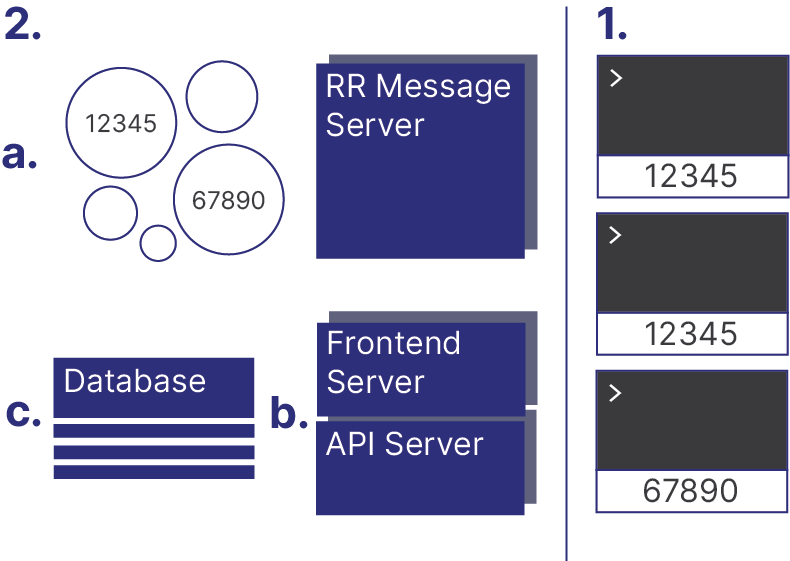
\includegraphics[scale=.8]{overall_system}
  \centering
  \caption{Overview of the Collaborative Debugger}
  \label{debugger:overview}
\end{figure}

The next sections give an overview of the various tools used to create
the collaborative debugger.  The debugger consists of:

\begin{enumerate}
\item A frontend web app built using React (\ref{react}) that presents
  a debugging interface to the end user.
\item A distributed backend managed by Kubernetes (\ref{k8s}), split
  into three parts:
  \begin{enumerate}
  \item A Pod for each debugging instance which runs the rr debugger
    (\ref{rr}).  These communicate directly with users through
    WebSocket server Pods. (\ref{socketio}).
  \item Pods running a frontend server written in Node.js which works
    in tandem with an API server created using Flask
    (\ref{flask/node}).  The API server manages creation and
    destruction of debug sessions, as well as authentication.
  \item A MongoDB (\ref{mongodb}) database.
  \end{enumerate}
\end{enumerate}

\subsection{Kubernetes}\label{k8s}

Kubernetes is the defacto standard in container orchestration
software.  It provides a layer of abstraction on top of normal
containers, like those created by Docker.  By bundling one or more
closely linked containers into a ``Pod'', Kubernetes is able to manage
deployment and re-deployment of applications running inside
containers.  It is trivial to create new Pods, or to create multiple
Pods running the same application as needed within a Kubernetes
cluster \cite{k8s}.  The speed at which even relatively large Pods can
be created and the inherent security provided by containerization
drove the decision to create a new Pod on the fly for each debugging
instance in the collaborative debugger.  This allows the debugger to
provide a similar level of convinience to exisiting collaborative
tools, such repl.it (\ref{exisitingcollab}).
\par

Kubernetes also provides services to facilitate load balancing, manage
storage volumes, and contain secrets.  The abstraction provided by
these features, in tandem with the ease of Kubernetes deployment on a
managed Kubernetes service\cite{do_managed_k8s} greatly accelerated
development.

\subsection{Mozilla's rr}\label{rr}

\subsubsection{Overview}

rr is ``a lightweight tool for recording, replaying and debugging
execution of applications''\cite{rr-repo}. rr allows a programmer to
record the execution of a program on any compatible machine and replay
the execution later.  This enhances GDB's ability to ``time-travel''
when debugging, using commands such as \lstinline{reverse-continue}
and \lstinline{reverse-stepi}\cite{gdbman} to step backwards and
forwards through a program's execution.  Through a novel encapsulation
of the execution space, rr is able to deterministically record and
replay the execution of syscalls and other process behavior that
differs run-to-run.  This is invaluable when trying to debug behavior
that is not entirely dependent on the code being debugged.  A typical
workflow in rr consists of recording an inexplicable error, replaying
execution to find the area in which the error occurs, and then
narrowing in on the bug not by re-running the entire program, but by
progressing back and forth through execution in the problem area.
\par

rr is an ideal tool for teaching debugging because it allows
instructors to record execution of a program and design a debugging
example with the knowledge that normally non-deterministic events will
be repeatable, and that any input they provide to the program will be
exactly replicated.  With the collaborative debugger, teachers can
record a program's execution and design a debugging lesson which
students can work on together.  The repeatability of rr means that
students can focus on debugging, and teachers can create as specific
examples as they please.  The use of rr is the most significant step
the collaborative debugger takes to addressing the lack of
back-tracing ability/coverage found in existing tools for teaching
debugging\cite{10.1145/3286960.3286970}.

\subsubsection{Limitations}

In comparison to solutions like PANDA\cite{10.1145/2843859.2843867}
that rely on capturing the entire state of of a virtual machine to
replay execution, rr records and replays faster, produces far smaller
files, and doesn't force execution inside of a
VM.\cite{DBLP:journals/corr/OCallahanJFHNP17} The trade off for these
benefits are two major system limitations: rr is only compatible with
the Linux kernel, and it's deterministic recording and replay relies
on a feature that is only found on modern \textit{Intel} x86 CPUs.
These limitations influenced the development of this project as a
webapp similar to existing tools for collaborative programming.
\par

Luckily, the speed and size benefits of rr lend themselves well to
non-local execution.  In conjunction with Kubernetes, it takes a few
seconds to create a new container running rr and connect to web
clients.

\subsection{pygdbmi}

In order to ``support the development of systems which use the
debugger as just one small component of a larger system'', GDB
provides a machine-oriented interface called GDB/MI \cite{gdbman}. rr
supports interaction through GDB/MI, and using the interface was a
natural choice for the collaborative debugger.  In addition to being
far easier to interact with from within a program, the structured,
machine-friendly output of GDB/MI lends itself in particular to future
development of visualization aids in the collaborative debugger.
\par
To parse rr output into Python dictionaries and to easily control rr
as a subprocess, pygdbmi \cite{pygdbmi} is used in each debugging Pod.
pygdbmi's abstraction simplifies programatically controlling rr.  A
Pod can receive a command from the client, pass it to rr, and respond
without having to deal with parsing GDB/MI output or with directly
managing the rr process.

\subsection{Socket.IO}\label{socketio}

To speed communication, the collaborative debugger uses WebSockets to
directly connect web clients and the Pods running rr.  Socket.IO is a
library that extends WebSockets.  It provides backup incase a
WebSocket connection cannot be established, enables automatic
reconnection and disconnection detection, and adds support for
namespaces \cite{socketio}.  The collaborative debugger uses the
standard JavaScript implementation of Socket.IO on the client side.
Messages are passed through a server to individual debugging Pods,
both of which use the Python implementation of Socket.IO,
python-socket.io \cite{python_socketio}.

\subsection{MongoDB}\label{mongodb}

The collaborative debugger uses a database to store information about
users, Pods, and example debugging sessions.  Due to it's speed of
deployment and natural interaction with the object-oriented languages
used to create the project, MongoDB was chosen as database software
\cite{mongodb}.

\subsection{Flask and Node.js}\label{flask/node}

The primary server for the collaborative debugger is split into two
sections: a simple Node.js \cite{node} server that serves the frontend
webapp, and an API server created using Flask \cite{flask}.  While in
development, the builtin React (\ref{react}) development server
is used to serve the frontend.  This makes debugging the frontend far
easier.
\par

An API server is necessary to authenticate users and to provide a
means to create/delete debugging sessions.  Since the rest of the
backend was created using Python, Flask was chosen to create the API
server.  Flask is a lightweight web application framework which lends
itself perfectly to interacting with the Python MongoDB and Kubernetes
APIs.

\subsection{React}\label{react}

React is JavaScript library that simplifies creating user interfaces
and managing state \cite{react}.  React's state management is of
particular importance to the collaborative debugger's frontend.  State
constantly changes as users create/delete debugging sessions, join
existing sessions, and communicate with rr.  React allows classes to
encapsulate components such as a list of existing debugging sessions,
a view of the current program's source code, and the terminal
interface with rr.  Instances of these classes maintain state
and update efficiently.
\par
The frontend makes extensive use of JSX, syntax which allows the
inclusion of segments of HTML code within a React app written in
JavaScript.  This makes it easy for each component of the one-page
webapp to hide/show subcomponents as state changes.

\subsection{Monaco and Xterm.js}\label{xtermjs/monaco}

After joining or creating a debugging session, users spend most of
their time interacting collaboratively with rr.  Their primary
interface to rr is through Xterm.js, a frontend component that makes
it easy to emulate terminal behavior in the browser \cite{xtermjs}.
With a few control methods, it is simple to provide a terminal
interface to rr that is virtually indistinguishable from a local
session.  By using the Xterm.js based interface, students can learn to
use rr (and by extension gdb) collaboratively, and directly translate
that knowledge to individual work.
\par

In addition to the terminal interface, the frontend shows a view of
the current source file being debugged.  The Monaco Editor
\cite{monaco} is used to display this source view.  Though more
complex than is strictly necessary to display code, Monaco makes it
easy to format and syntax-highlight.  Using Monaco also simplifies the
future addition of editing source code, should the need arise.
React's state management allows updating text in the editor as
efficiently as possible.

\section{Design}

The collaborative debugger consists of a distributed Kubernetes
backend and frontend React webapp.  Kubernetes was chosen for the
backend primarally so that a Pod could be created dynamically for each
debugging session.  The design of the backend is heavily distributed,
allowing individual components to be modified without the whole system
needing to be reconfigured.

\begin{figure}[h!]

  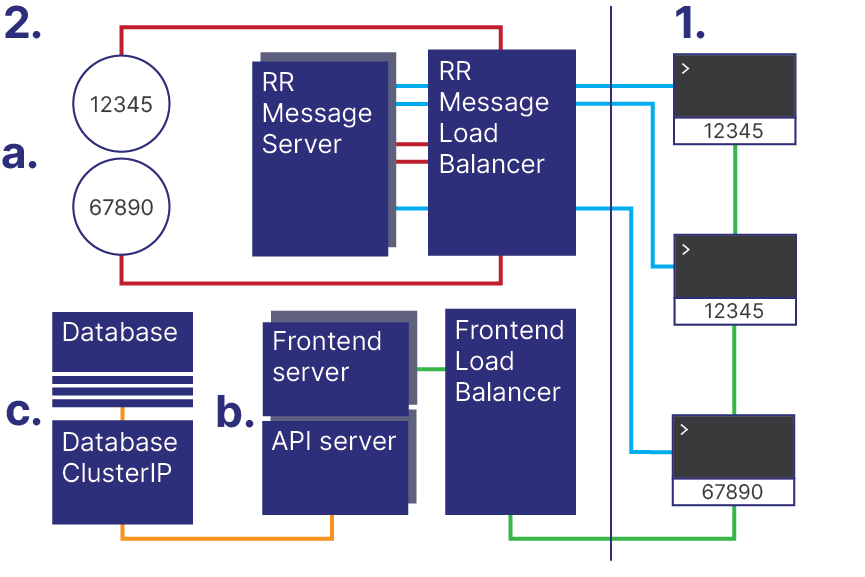
\includegraphics[scale=.9]{detailed_system}
  \centering
  \caption{Detailed Overview of the Collaborative Debugger}
  \label{debugger:detailedoverview}
\end{figure}

Each backend component of the collaborative debugger runs in it's own
individual Pod.  There are two different classes of Pods in the
collaborative debugger:

\begin{enumerate}
\item Statically created Pods.  These are the \textit{RR Message
    Server Pods}, the \textit{Frontend/API Server Pods}, and the
  \textit{Database Pod}.  This class of Pods are manually created when
  the cluster that will run the backend is first initialized.  The RR
  Message Server Pods and Frontend/API Server Pods may be created
  using Deployments \cite{k8s_docs} to allow later scaling, where
  multiple Pods running the same application may be created to
  facilitate increased load.
\item Dynamically created Pods.  This class of Pod contains the
  individual instances of \textit{RR Debug Session Pods} that are
  created on request by the API server.  When a client requests a new
  debug session, the API server uses the Kubernetes API to create a
  new Pod based on an existing template, gives the Pod a unique
  identifier, and associates it in the database with the requesting
  client.
\end{enumerate}

These Pods communicate with other Pods in the cluster and with the
outside world through Services.  The Kubernetes documentation defines
a Service as ``an abstraction which defines a logical set of Pods and
a policy by which to access them'' \cite{k8s_docs}.  In the
collaborative debugger, these Services manifest as:

\begin{enumerate}
\item The \textit{Database ClusterIP}: a ClusterIP, which exposes the
  Database Pod only inside the cluster.  The only component that makes
  use of this ClusterIP is the API server, which uses it primarily to
  communicate information about users and RR Debug Sessions with the
  database.
\item The \textit{RR Message Load Balancer}: a Load Balancer, which
  exposes the RR Message Server Pods to the outside world.  Using
  Socket.IO, clients send commands to and recieve responses from
  individual RR Debug Session Pods through the RR Message Server Pods.
\item The \textit{Frontend Load Balancer}: another Load Balancer,
  which exposes the Frontend/API Server Pods to the outside world.
  Clients request the frontend webapp and send api requests/recieve
  api responses through this Load Balancer.
\end{enumerate}

The frontend webapp dynamically updates as the user requests new debug
sessions, issues commands to rr, and visits new source files.  A user
can be part of multiple debug sessions simultaneously.  Each debug
session is assigned at 5 digit identifier at creation, which is used
to join sessions in progress.
\par

Each component of the backend and frontend will be discussed in depth
in the following sections.

\subsection{Configuration and Setup}

Configuration and setup of the collaborative debugger is relatively
simple.  After a Kubernetes cluster is created (this is made easier by
using a Managed Kubernetes service) Pods and Services are created
using various configuration files.  Services should be created first,
so that Pods which rely on access to Services function properly on
creation.  The following sections outline the process of creating a
cluster, Pods, and Services, with a focus on statically created Pods.
The process of building images for building dynamically created Pods
is similar, but the process of starting the Pods is more complicated.
This process will be discussed in-depth in the section on the API
server (\ref{api}).

\subsubsection{Cluster Selection and Configuration}

Though Kubernetes aims to be largely platform-agnostic, the
requirements of rr impose some restrictions on cluster setup and
configuration.  Clusters, even those running inside a VM, must be run
on machines using relatively modern Intel x86 CPUs (Nehalem and
beyond).  The clusters must run on an operating system using Linux
kernel version 3.11 or higher \cite{rr-repo}.  Finally, in order for
rr to be able to work efficiently, the
\lstinline{kernel.perf_event_paranoid} parameter must be set to 1
\cite{rr-repo}.  This should be done on every node in the cluster
which will run RR Debug Sessions.  For the purposes of development, it
has been set to 1 on all nodes in the collaborative debugger cluster.

\subsubsection{Creating Pods}

\begin{figure}[h!]

  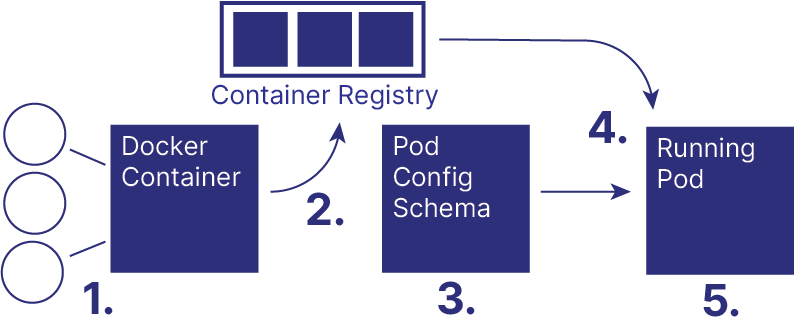
\includegraphics[scale=.9]{pod_creation}
  \centering
  \caption{The Pod Creation Process}
  \label{podcreation:overview}
\end{figure}

Pods are created in five steps:

\begin{enumerate}
\item A \lstinline{Dockerfile} is used to build a new Docker container
  image from various pieces of source code, scripts, and a base image
  (such as the official MongoDB image or official Ubuntu image).  The
  Dockerfile also contains instructions to install necessary packages,
  run build scripts, and create file structures in the image.
\item The Docker image is tagged and uploaded to a private container
  registry.
\item A Pod configuration schema is defined/updated with details of
  the corresponding image's tag and any necessary Pod-specific
  settings/startup commands.
\item The Pod configuration schema is applied, either statically or
  dynamically.  When the schema is applied, Kubernetes pulls the image
  from the container registry and creates a new Pod according to the
  schema, running any startup commands if provided.
\item If Pod creation is successful, the result is a new Pod running
  in the cluster.
\end{enumerate}

\paragraph{1. Docker Container Creation}

Docker containers are created using a Dockerfile.  The Dockerfile used
to create the container image for the RR Message
Server is shown below:

\begin{lstlisting}[language=Dockerfile,caption={RR Message Server Dockerfile},captionpos=b]
# Base Image
FROM  ubuntu:latest

# Package Installation
WORKDIR /tmp/
ENV DEBIAN_FRONTEND="noninteractive"
RUN apt-get update && apt-get install -y \
python3-pexpect python3-pip

# User Creation
RUN useradd -ms /bin/bash rrserver
USER rrserver

# File structure creation/app setup
RUN pip3 install requests python-socketio \
eventlet
WORKDIR /home/rrserver/
RUN mkdir app
WORKDIR /home/rrserver/app/
COPY server.py .
COPY startup.sh .

# Startup command
CMD ["sh", "startup.sh"]
\end{lstlisting}

The build process for each collaborative debugger Docker image follows
the same structure as the one outlined in the Dockerfile above:

\begin{enumerate}
\item The base image is defined. The RR Message Server and RR Debug
  Session images are based on the latest Ubuntu image.  This is
  particuarly necessary for the RR Debug Session image, as rr's
  low-level nature necessitates somewhat frequent updates as changes
  are made to the Linux kernel.  The Frontend/API Server image is
  based on the latest Node image, and the Database image is based on
  the latest MongoDB image.
\item Second, any necessary packages are installed.  For the RR Debug
  Pod image, rr is compiled from source and installed.
\item A non-root user is created if necessary.
\item Program files are copied over and a file structure is created.
  Packages that don't rely on the base images builtin package manager
  are installed at this time.  In the example above, these include
  Python packages.
\item A startup command is defined.
\end{enumerate}

Each line in a Dockerfile corresponds to a layer in the built image.
This build order minimizes the amount of rebuilding necessary by
placing the items that are most likely to change towards the end of
the build process.

\paragraph{2. Container Registry Upload}

Most Managed Kubernetes services come with the option to create a
private container registry.  With proper authentication, this allows
Docker and Kubernetes to access user-created images as easily as if
they were in a public registry.  Images built with Docker are uploaded
to a private container registry for use in the collaborative debugger.

\paragraph{3. Pod Configuration Schema} \label{podschema}

The Pod configuration schema for most Pods in the collaborative
debugger is fairly generic.  It consists of a \lstinline{name}, an
\lstinline{image} sourced from the container registry, and in the case
of pods that need to interact with a load balancer, an
\lstinline{app}.

\begin{lstlisting}[language=YAML,basicstyle=\linespread{0.5}\ttfamily,caption={RR Debug Session Schema},captionpos=b]
apiVersion: v1
kind: Pod
metadata:
  name: rr-translation
  labels:
    purpose: translate-rr
spec:
  containers:
  - name: rr-test-container
    image: example-container-registry.com/sproj/...
    securityContext:
      capabilities:
        add:
        - SYS_PTRACE
  restartPolicy: OnFailure
\end{lstlisting}

A notable exception is the RR Debug Session Schema, which adds the
\lstinline{SYS_PTRACE} capability to the Pod.  This is necessary for
rr to properly trace system calls.

\paragraph{4 \& 5. Pod Creation}

For statically created Pods, the \lstinline{kubectl apply} command is
used to create new Pods.  Kubernetes pulls the container image defined
in the schema from the container registry and starts the Pod with any
necessary commands.  The database Pod is connected to a long-term
storage volume at this time.  Upon successful creation, the Pod is
ready to interact with any necessary load balancers.

\subsubsection{Service Creation}

Services are the first components of the collaborative debugger
created after the cluster is initiallized.  The three Services used by
the debugger are all statically created.  Like statically created
Pods, schemas that define Services are applied manually using the
\lstinline{kubectl apply} command.

\begin{lstlisting}[language=YAML,basicstyle=\linespread{0.5}\ttfamily,caption={Frontend Load Balancer Schema},captionpos=b]
apiVersion: v1
kind: Service
metadata:
  name: frontend-load-balancer
spec:
  selector:
    app: frontend
  type: LoadBalancer
  ports:
    - port: 3000
    targetPort: 3000
\end{lstlisting}

The \lstinline{app} field in the above schema corresponds to the
\lstinline{app} field defined in the metadata of the Frontend/API
Server configuration schema.  Traffic to the Load Balancer's external
IP address on port 3000 is redirected automatically by Kubernetes to
any Pod running the Frontend/API Server.  The Load Balancer determines
which Pod is the most suitable given current demands on the system.

\subsection{RR Debug Sessions \& RR Message Server}

At the heart of the collaborative debugger is the RR Debug Session.
Every time a user wants to debug a new program execution, an RR Debug
Session Pod is dynamically created by the API server.  The new Pod is
assigned a unique five digit identification number when it is created.
This five digit number, is used as the channel for the RR Debug
Session, seperating its communication from other RR Debug Session
Pods.  Clients, RR Message Server Pods, and the RR Debug Session Pod
connect through the RR Message Load Balancer.  Clients and RR Debug
Sessions send messages using the channel assigned to the pod at
creation time.  A diagram of one full communication cycle between two
clients and an RR Debug Session Pod is outlined in the diagram below:

\begin{figure}[h!]

  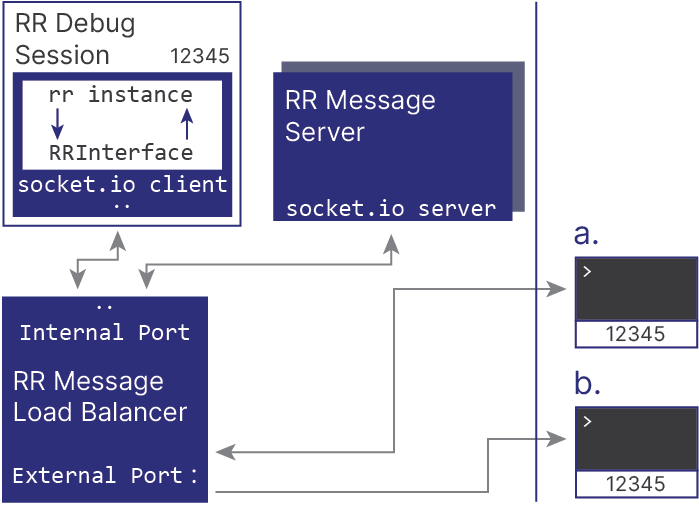
\includegraphics[scale=1]{rr_detailed}
  \centering
  \caption{RR Message Server Communication Cycle}
  \label{rr:detailed}
\end{figure}

The process of sending a command to an RR Debug Session and receiving
a response is as follows:

\begin{enumerate}
\item Client A, already having connected to the channel that
  corresponds to it's current RR Debug Session (channel 12345 in the
  example), sends an rr command.
\item The RR Message Server recieves the command and emits a message
  that RR Debug Session Pods are equiped to recieve on the same
  channel.  In practice, since only one RR Debug Session Pod is ever
  on a channel, this equates to emmiting a message to the Pod
  directly.
\item The RR Debug Session Pod recieves the message, and passes the
  command to its instance of RRInterface.  When it recieves a
  response, it emits the output from rr along with other debugging
  information and the channel.
\item The RR Message Server recieves the response, and emits a
  response message that clients are equipped to recieve on the
  corresponding channel.
\item Clients A and B are connected to the corresponding channel, so
  they both recieve the response.
\end{enumerate}

\subsubsection{RR Message Server}

The RR Message server is remarkably simple, consisting of just 3
important functions:

\begin{lstlisting}[language=Python,basicstyle=\linespread{0.5}\ttfamily,caption={RR Message Server},captionpos=b]
@sio.on('join_channel')
def join_channel(sid, data):
    sio.enter_room(sid, data['channel'])

@sio.on('rr_command')
def on_rr_command(sid, data):
    data['sid'] = sid
    try:
        sio.emit('rr_command', data,
                 room=data['channel'])
    except:
        pass

@sio.on('rr_response')
def on_rr_response(sid, data):
    sio.emit('rr_response', data,
             room=data['channel'])
\end{lstlisting}

Even in a fully production ready version of the collaborative debugger
with more security features enabled, the RR Message Server is unlikely
to become much more complex.  It exists purely to pass messages
between clients and RR Debug Session Pods and to manage channels.
Since the design of other aspects of the collaborative debugger ensure
that all members of a given channel exist only during the lifetime of
it's corresponding RR Debug Session Pod, the
\lstinline{'join_channel'} event handler simply adds socket.io clients
to a specified channel on request.
\par

The two message processing functions, \lstinline{on_rr_command} and
\lstinline{on_rr_response}, are equally simple.  When the RR Message
Server recieves an \lstinline{'rr_command'} message, it passes the
message data along to the corresponding RR Debug Session Pod by
emitting an \lstinline{'rr_command'} namespaced to the correct channel
with \lstinline{room=data['channel']}.  Since the socket.io client
running in RR Message Server Pods has an event handler defined for
\lstinline{'rr_command'}s but frontend clients do not, only RR Message
Server Pods recieve the command.  The same process happens in reverse
for \lstinline{'rr_response'}s, with only the frontend socket.io
clients having a handler defined for \lstinline{'rr_response'}.


\subsubsection{RR Debug Session}

\paragraph{Building Example Pods} \label{buildingchannel}

The process for building RR Debug Session example images is differs
slightly from other images used by the collaborative debugger.
Currently, three example RR Debug Session images are availiable for
use.  Example container images are based on the primary RR Debug
Session image, RR Translation.  The build process for this image,
based on the lasted official Ubuntu container image, installs rr,
python, and all necessary packages as well as the app that will run on
the final image, \lstinline{rrtranslation.py}.

\begin{lstlisting}[language=Dockerfile,basicstyle=,caption={RR Debug Session Hash Example---Dockerfile},captionpos=b]
FROM example-container-registry.com/sproj/...
  
WORKDIR /home/debug/app/
COPY hash.c .
COPY names .
COPY startup.sh .
\end{lstlisting}

The Dockerfile shown above is for a simple hash program RR Debug
Session example.  The build process copies over any necessary files,
as well as a startup script:

\begin{lstlisting}[basicstyle=\linespread{0.5}\ttfamily,caption={Example Startup Script},captionpos=b]
gcc -g -o hash hash.c
rr record ./hash
python3 rrtranslation.py $1
\end{lstlisting}

This script is used to start the \lstinline{'rrtranslation.py'} program
when the Pod is dynamically created.  The script will be passed the
Pod's channel as argument \lstinline{$1} by the Kubernetes API on
startup.
\par

Current example pod startup scripts compile the program to be debugged
and record execution when the pod is created.  It is easy to create a
more specific example to be replayed, if exact reproduction of
syscalls or other non-deterministic behavior is desired.  The
example's creator can record an rr session locally ahead of building
the example Pod and copy the recording into the appropriate folder
during the build process.  Since rr recordings are portable, the
example will replay without issue in the RR Debug Session Pod.

\paragraph{The RR Translation Program} \label{joiningchannel}

The RR Translation program consists of two main components: a socket.io
client, \lstinline{sio}, and an instance of the
\lstinline{RRInterface} class, \lstinline{rri}, that controls the rr
subprocess and parses interactions.  Simple code to read information
about the current source file currently exists within
\lstinline{sio}'s \lstinline{'rr_command'} event handler, but should
be broken out into its own class if more complexity is added.
\par

The RR Translation program's socket.io client instance begins by
connecting to the RR Message Server.  It immediately emits a
\lstinline{'join_channel'} message, using the channel passed in from
the Kubernetes API call on it's creation. 

\begin{lstlisting}[language=Python,basicstyle=\linespread{0.5}\ttfamily,caption={RR Translation Main},captionpos=b]
if __name__ == '__main__':
    channel = sys.argv[1]
    sio.connect('http://rr-message-server-load-balancer:8000')
    sio.emit('join_channel', {'channel': channel})
\end{lstlisting}

After joining the appropriate channel, \lstinline{sio} waits to
recieve an \lstinline{'rr_command'}.  The first part of
\lstinline{sio}'s \lstinline{'rr_command'} event handler is shown below:

\begin{lstlisting}[language=Python,basicstyle=\linespread{0.5}\ttfamily,caption={RR Command Event Handler},captionpos=b]
@sio.on('rr_command')
def on_rr_command(data):

    body = {'from': data['sid'],
            'command': data['command'],
            'channel': channel}
    
    try:
        response = {'output': rri.write(data['command'])}
\end{lstlisting}

The handler first builds part of the response body, passing back data
about the channel and originator of the message that will be important
for the RR Message Server and client later.  Next, it calls the
function necessary to pass a message to rr and recieve a response,
\lstinline{rri.write()}.
\par

When the program starts, an instance of the \lstinline{RRInterface}
class, \lstinline{rri}, is initialized in the same scope as
\lstinline{sio}.  \lstinline{RRInterface} contains an instance of the
\lstinline{GDBController} class from pygdbmi to interface with rr and
control the rr subprocess, as well as a collection of methods to parse
rr output, the three most important of which are shown below: 

\begin{lstlisting}[language=Python,basicstyle=\linespread{0.5}\ttfamily,caption={RRInterface},captionpos=b]
def get_full_rr_response(self, command):
    response = self.gdbmi.write(command)
    while(not(self.end(response) or self.exited(response))):
        response.extend(self.get_rr_response())
    return response

def write(self, command):
    if self.command_forbidden(command):
        raise DissallowedError
    self.timeline.append(command)
    return self.console_output(
        self.get_full_rr_response(command))

def source(self):
    f = self.get_full_rr_response(
        '-file-list-exec-source-file')[0]['payload']
    return {'file': f['file'],
            'line': f['line'],
            'path': f['fullname']}
\end{lstlisting}

When \lstinline{write} is called, it determines if the command to be
executed is forbidden.  Currently only one gdb command,
\lstinline{shell}, is disallowed.  Parsing the output from
\lstinline{shell} is difficult, it is of virtually no use since
\textit{recordings}, not currently executing programs that
\lstinline{shell} could effect are being debugged, and it opens the
door to security issues.  Though containerization means that the most
users could probably do is render their own debug session useless, the
downsides of \lstinline{shell} far outweigh the benefits.
\par

Next, write appends the command to the \lstinline{RRInterface}'s
\lstinline{timline} instance variable.  \lstinline{timeline} is a list
of all commands the debug session has executed.  Though unused at the
moment, it can serve in the future to impliment a shared history
between all clients and to facilitate the saving of debug sessions
in-progress.  By issuing all commands in \lstinline{timeline} to a new
instance of \lstinline{RRInterface} with the same recording, it is
possible to restore a debug session to an identical previous state.
To save a debug session, the recording and \lstinline{timeline} can be
stored in a database, and be used to initialize a new Pod with
identical state to a previous RR Debug Session Pod.  This appears to
clients as a seemless restoration of a previous Debug Session.
\par

Since the frontend currently consists of a terminal interface to rr
and a view of the current source code, write does not need to return
any information from rr other than console output.  Future versions of
the collaborative debugger that support visualization tools could use
gdbmi commands such as \lstinline{-stack-list-frames} to retrieve
information to be used by frontend visualization tools.
\lstinline{console_output} extracts user-relevant output from the
dictionary returned by \lstinline{GDBController}'s \lstinline{write}
method.  The \lstinline{get_full_rr_response} method ensures that all
relavant output has been recieved from the rr subprocess before
returning.  Write reduces the lengthy dictionary that would be
produced by a command as simple as \lstinline{break main} into a few
lines of user-relevant output.
\par

After the \lstinline{'rr_command'} event handler has recieved a
response from \lstinline{rri}, it calls \lstinline{RRInterface}'s
\lstinline{source} function to retrieve information about the current
source file being debugged.  Most often the source file has not
changed, and the only relevant piece of information that needs to be
passed back to the client is the new line number in the source file.
If the source file has changed, the handler reads its contents,
updates \lstinline{current_file}, and emits the line number, file
name, and contents.  If an error occurs at any point in the process, a
detailed trace is emmitted for debugging purposes.  The trace should
be ommited in production.
\par

Most of the complexity in the RR Translation program stems from
parsing rr output.  The flow of data in the program is quite simple: a
command is recieved, it is passed to rr, rr's response is processed,
and a response message is emmited.  This flow would remain unchanged
even with the addition of functions to retrieve information for data
visualization.  Since the process of turning rr responses into a
terminal interface takes place in the frontend, rather than the RR
Translation program providing some sort of REPL over WebSockets,
updates can be made to the frontend webapp without requiring backend
changes.  The whole process is also quite snappy, with only a slight
delay from the client's perspective compared to running a debugger
natively.
\par

Effort is taken in the design of the RR Debug Session and RR Message
Server to ensure students recieve a pleasant and near-identical
experience to debugging locally in the future.  The system of
inheritance used to create example debug session pods is designed to
be as simple as possible, though a more fully featured frontend could
simplify this process further in the future.

\subsection{Frontend/API Server}\label{api}

The second major backend system consists of the Frontend/API Server
and database.  This system is responsible for serving the frontend
webapp, as well as processing all API requests, such as those to
authenticate users and create new RR Debug Sessions.  The builtin
React development server is used to serve the frontend webapp and
redirect API requests to the Flask API server during development.  For
both security and performance reasons this should be changed to a
combination of a more robust solution like Nginx \cite{nginx} and a
production suitable web server for production.  The relationships
between components and overall process will remain unchanged after
this migration.
\par

Since the entire webapp is one page, the process for serving it is
completely standard.  The server recieves a request for the index page
of the website, and returns the compiled React webapp that makes up
the homepage.  The process for API requests is more involved, and an
example is outlined below:

\begin{figure}[h!]

  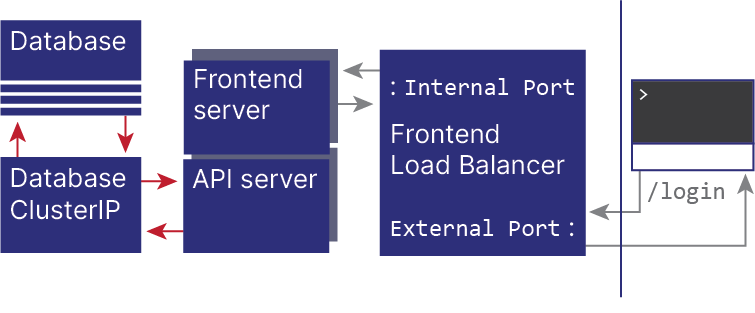
\includegraphics[scale=1]{login_request}
  \centering
  \caption{API Request Process---Login}
  \label{rr:detailed}
\end{figure}

\begin{enumerate}
\item The client makes a POST request to the \lstinline{'/login'} URL.
  This request contains the necessary data to log in the user.
\item The frontend server forwards the request of a URL it does not
  recognize to the API server running in the same Pod on a different
  port.
\item The API server recognizes the \lstinline{'/login'} route, and
  communicates with the database to attempt to log in the user.
\item The API server returns the result of the login request, which is
  returned by the frontend server to the client.
\end{enumerate}

\subsubsection{Frontend/API Server Configuration}

The Frontend/API Server uses Yarn \cite{yarn} to manage packages.
When a Frontend/API Server Pod is deployed, the Pod's startup script
uses the \lstinline{yarn start} and \lstinline{yarn start-api}
commands to start the frontend server and API server respectively.
These scripts are defined in the server's \lstinline{package.json}
configuration file:

\begin{lstlisting}[basicstyle=\linespread{0.5}\ttfamily,caption={Frontend/API Server Configuration},captionpos=b]
  "start": "react-scripts start",
  "start-api": "cd api && flask run --no-debugger",
  .
  .
  .
  "proxy": "http://localhost:5000",
\end{lstlisting}

Also of note in \lstinline{package.json} is the instruction to proxy
the API server, which is running on port 5000.  This achieves the
automatic forwarding of API requests to the API server described
above.  Since API requests are proxied through the same address
serving the frontend webapp, there are no issues with cross-origin
requests.

\subsubsection{The API Server}

The API server is implimented using Flask.  The server program
consists of handlers for the various API routes and instances of two
classes which communicate with the database/Kubernetes API:
\lstinline{TranslationPodManager} and \lstinline{UserManager}.  The
full structure of the API Server program, \lstinline{api.py} is shown
below:

\begin{figure}[h!]

  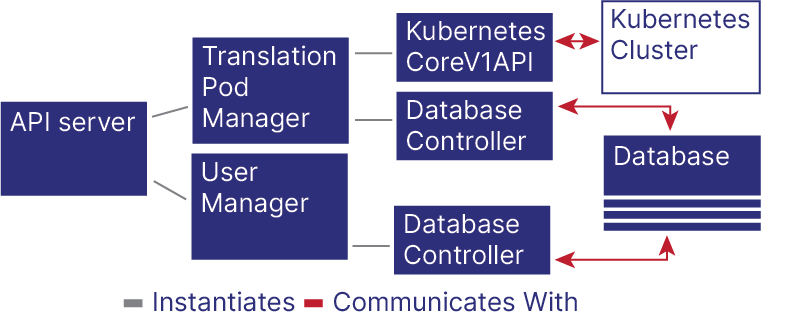
\includegraphics[scale=1]{api_structure}
  \centering
  \caption{Structure of the API Server}
  \label{rr:detailed}
\end{figure}

Care was taken to abstract as much as possible in the design of the
API server and the classes it instantiates.  The two classes
instantiated by \lstinline{api.py}, \lstinline{TranslationPodManager}
and \lstinline{UserManager}, each instantiate another class which
interacts with the database, \lstinline{DatabaseController}, as an
instance variable.  \lstinline{TranslationPodManager} further
instantiates the Kubernetes Core V1 Python API to communicate with the
cluster in order to create/delete pods.  This process of abstraction
ensures that the database, underlying cluster structure, and
authentication methods can all change without significant changes
needing to be made to \lstinline{api.py}.
\par

The most significant improvement that could be made to this structure
would be to break the \lstinline{UserManager} and
\lstinline{TranslationPodManager} instances out into seperate programs
running on their own Pods in the cluster.  This would allow changes to
be made in those classes, say to update the process of deleting Pods,
without needing to update the entire Frontend/API Server Pod.  For the
time being, the relative simplicity of the API means that the added
complexity and overhead of implementing a method to communicate
between dedicated \lstinline{TranslationPodManager} and
\lstinline{UserManager} Pods and Pods running the Frontend/API Server
doesn't seem worthwhile.  This may change in the future.
\par

Currently supported API requests are as follows:

\begin{enumerate}
\item \lstinline{'/login'}: Logs in the user given by
  \lstinline{'name'}, or, (given the rather lax development security)
  creates a user if none matching \lstinline{'name'} exists.  Returns
  the name of the user.
\item \lstinline{'/channel'}: How users join RR Debug Sessions.  Binds
  the user given by \lstinline{'name'} to an RR Debug Session Pod
  matching \lstinline{'channel'} in the database, if such a Pod
  exists.  Returns the channel.
\item \lstinline{'/pods'}: How the client gets a list of RR Debug
  Session Pods the user is currently participating in.  Returns the
  channels for all RR Debug Session Pods who the user, given by
  \lstinline{'name'}, is currently bound to in the database.
\item \lstinline{'/examples}: How the client gets a list of example RR
  Debug Session Pod names.  Returns all names of example RR Debug
  Session Pods that exist in the database.
\item \lstinline{'/new'}: Creates a new RR Debug Session Pod based on
  the name given by \lstinline{'program'}.  Binds the user, given by
  \lstinline{'name'}, to the Pod.  Returns the channel of the Pod.
  This request is the most complex, and is covered in more detail
  below.
\item \lstinline{'/delete'}: Deletes a binding between the user given
  by \lstinline{'name'} and the RR Debug Session Pod given by
  \lstinline{'channel'}.  If there are no bindings left between the
  Pod and users (if all the users have left the debug session),
  deletes the Pod from the database and the cluster.  Returns
  \lstinline{True}.
\end{enumerate}

All the API request handlers listed above return an error message in
the case of an error occuring during the processing of an API request.
Since most errors that could occur would either be the result of
unanticipated issues on the part of the user, or of some unforseen
catostrophic internal error, informing users of error specifics would
be unhelpful.  Some \lstinline{TranslationPodManager} and
\lstinline{UserManager} functions throw specific errors in the event
of duplicate usernames, channels that do not exist, etc.  These errors
are caught and meaningful error messages are returned to the frontend
webapp, which can then pass them on to the user.
\par

To examine the process of processing an API request, it makes sense to
look at the most complex example, creating a new RR Debug Session Pod.
This example shows the process for processing an API POST request,
interacting with the database, and dynamically creating a Pod.  All
API requests follow a similar procedure.

\paragraph{Processing a POST Request---Extracting Information}

Below is the route handler for the \lstinline{'/new'} URL, as well as
the instantiation of \lstinline{TranslationPodManager} and
\lstinline{UserManager}.

\begin{lstlisting}[language=Python,basicstyle=\linespread{0.5}\ttfamily,caption={API Server New RR Debug Session Event Handler},captionpos=b]
tpm = podmanager.TranslationPodManager(
                   url='mongodb://database-load-balancer',
                   port=27017)
um = usermanager.UserManager(
                   url='mongodb://database-load-balancer',
                   port=27017)
app = Flask(__name__)

@app.route('/new', methods=['POST'])
def new():
    try:
        name = request.get_json()['name']
        program = request.get_json()['program']
        channel = tpm.create_pod([name], program)
        return {'channel': channel}
    except:
        return {'error': 'Internal Error'}
\end{lstlisting}

All API routes only support POST requests.  The route handler first
extracts the relavant information from the POST request body, in this
case \lstinline{name} and \lstinline{program}.  \lstinline{name}
always corresponds the user who is making the request's username, and
\lstinline{program} corresponds to the name of the example RR Debug
Session image to be used.
\par

\lstinline{new} then calls \lstinline{TranslationPodManager}'s
\lstinline{create_pod} function to create a new RR Debug Session Pod.
\lstinline{create_pod} can bind multiple users to a Pod when it is
created, so \lstinline{name} is passed inside a list.

\paragraph{The Database} Before drilling into \lstinline{create_pod},
it may be helpful to examine the MongoDB database which
\lstinline{TranslationPodManager} and \lstinline{UserManager} interact
with.  The database consists of three collections: \lstinline{users},
\lstinline{pods}, and \lstinline{examples}.  Below is an example
record from each collection:

\begin{figure}[h!]

  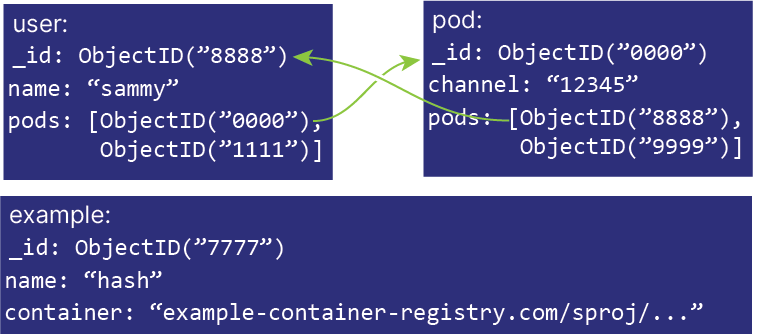
\includegraphics[scale=1]{database_example}
  \centering
  \caption{Database Record Examples}
  \label{rr:detailed}
\end{figure}

\lstinline{pods} and \lstinline{users} have a many-to-many
relationship.  Each user can be bound to an unlimited number of pods,
and vice versa.  The \lstinline{DatabaseController} class includes
functions to efficiently retrieve \lstinline{users} and
\lstinline{pods} given one another, and to create/destroy bindings
between \lstinline{users} and \lstinline{pods}.
\par

\lstinline{examples} are independent of \lstinline{users} and
\lstinline{pods}.  The continer registry URLs of RR Debug Session
example images are stored in the database so that new images can be
easily added to the collaborative debugger upon creation.
\par

MongoDB keeps \lstinline{_id}s unique.  In addition, the collaborative
debugger defines uniqueness constrains on \lstinline{users:name},
\lstinline{pods:channel}, and \lstinline{examples:name} when the
database is created.

% \begin{lstlisting}[basicstyle=\linespread{0.5}\ttfamily,caption={Frontend/API Server Configuration},captionpos=b]
% users:            pods:               examples:
%   _id ObjectId      _id ObjectId        _id ObjectId
%   name String       channel String      name String
%   pods Array        users Array         container String

% Example user:
% {
% 	"_id" : ObjectId("5fc14c622dc45448d67189b3"),
% 	"name" : "sammy",
% 	"pods" : [
% 		ObjectId("5fc14d5b2dc45448d67189b4"),
% 		ObjectId("5fc59acb2dc45448d67189b6")
% 	]
% }

% Example pod:
% {
% 	"_id" : ObjectId("5fc14d5b2dc45448d67189b4"),
% 	"channel" : "19452",
% 	"users" : [
% 		ObjectId("5fc14c622dc45448d67189b3"),
% 		ObjectId("5fc317d22dc45448d67189b5")
% 	]
% }

% Example example:
% {
% 	"_id" : ObjectId("5fc14d50b92a752776d3fd7d"),
% 	"name" : "hash",
% 	"container" : "example-container-registry.com/sproj/..."
% }
% \end{lstlisting}

\paragraph{Processing a POST Request---Dynamic Pod Creation}

To dynamically create a Pod, \lstinline{create_pod} gets the container
registry URL of the image to base the Pod on, creates the new Pod,
binds users to the Pod, and returns the channel the Pod was created
with.  The first part of the function is shown below:

\begin{lstlisting}[language=Python,basicstyle=\linespread{0.5}\ttfamily,caption={Pod Creation 1},captionpos=b]
def create_pod(self, names, program):
  examples = self.get_examples()
  image = None
  try:
    image = examples[program]
  except:
    raise NoSuchExampleError
\end{lstlisting}

\lstinline{create_pod} calls \lstinline{TranslationPodManager}'s
\lstinline{get_examples} method to get a list of RR Debug Session
example image names and container registry URLs from the database.  In
the event that the user has somehow pased a spurious image name or has
passed a name when there are no images, an exception is raised.
Otherwise, a RR Debug Session Pod schema is created using the image:


\begin{lstlisting}[language=Python,basicstyle=\linespread{0.5}\ttfamily,caption={Pod Creation 2},captionpos=b]
  dep = {'apiVersion': 'v1',
         'kind': 'Pod',
         'metadata': {'labels':
                      {'purpose': 'translate-rr'}},
         'spec': {'containers':
                  [{'image': image,
                    'name': 'rr-test-container',
                    'command': ['sh'],
                    'args': ['startup.sh'],
                    'securityContext':
                    {'capabilities':
                     {'add': ['SYS_PTRACE']}}}],
                   'restartPolicy': 'OnFailure'}}
\end{lstlisting}

This schema, represented as a dictionary in Python, is identical to
the YAML representation of the RR Debug Session Pod creation schema
shown in (\ref{podschema}) with the exception of \lstinline{args}
which will be updated further in a later step.  Finally,
\lstinline{create_pod} does the
work necessary to dynamically create a Pod:

\begin{lstlisting}[language=Python,basicstyle=\linespread{0.5}\ttfamily,caption={Pod Creation 3},captionpos=b]
  channel = self.dbc.add_pod(
            self.dbc.get_userids_by_name(names))
  dep['metadata']['name'] = channel
  dep['spec']['containers'][0]['args'].append(channel)
  resp = self.v1.create_namespaced_pod(
         body=dep, namespace='default')
  # Wait to return the channel until the pod is live
  # and read to recieve incomming communication
  status = self.v1.read_namespaced_pod_status(
           channel, 'default').status.container_statuses
  while status == None or status[0].state.running == None:
    time.sleep(1)
    status = self.v1.read_namespaced_pod_status(
             channel, 'default').status.container_statuses
  return channel
\end{lstlisting}

First, \lstinline{DatabaseController}'s \lstinline{add_pod} method is
called to insert a new \lstinline{pods} record into the database.
\lstinline{add_pod} randomly generates a new five digit
\lstinline{channel} for the Pod, using the uniqueness constraint
imposed on \lstinline{pods:channel} to ensure an unused
\lstinline{channel} is generated.  If no channels are open an error is
raised.  Otherwise, the users passed to \lstinline{add_pod} are bound
to the new Pod in the database, and \lstinline{channel} is returned.
This process has the effect of limiting the number of simultaneous RR
Debug Sessions that can be in use at the same time to 89999, and of
slowing as more channels are used.  Given the few current users, the
likelyhood of a collision when generating a new channel is low enough
that a more advanced method is unnecessary.
\par

Next, the name of the container is updated to \lstinline{channel}.  In
addition, the startup arguments are updated to include
\lstinline{channel}.  This is how \lstinline{channel} is passed to the
\lstinline{startup.sh} script and eventually used to join a channel on
the RR Message Server in \lstinline{rrtranslation.py}
(\ref{buildingchannel} \& \ref{joiningchannel}).
\par

The Kubernetes API is then finally used to create the Pod.  The Pod is
created in the default namespace.  This could be changed to logically
isolate dynamically and statically created Pods with minimal hassle,
since Kubernetes' DNS resolution can connect pods accros namespaces.
If Pod creation fails, an error will be thrown.  Otherwise, a loop is
used to wait until \lstinline{rrtranslation.py} is running inside the
Pod.  Once the Pod is ready, \lstinline{channel} is returned.

\paragraph{Processing a POST Request---Returning a Response}

Most request handlers, \lstinline{'/new'} included, simply return a
JSON serializable dicitionary containing whatever results the API
Server's instance of \lstinline{TranslationPodManager} or
\lstinline{UserManager} returned, or an error message.  The
\lstinline{'/new'} handler returns \lstinline{'channel': channel} so
that the frontend webapp's socket.io client can join the channel
corresponding to the RR Debug Session Pod that was just created.

\subsection{Webapp}\label{webapp}

TODO

\section{Next Steps}

TODO

\pagebreak
\bibliographystyle{acm}
\bibliography{sprojbib}{}
\end{document}
